\newpage
\section{顾客端AI功能}
\label{sec:guest_features}

\begin{figure}[htbp]
	\centering
	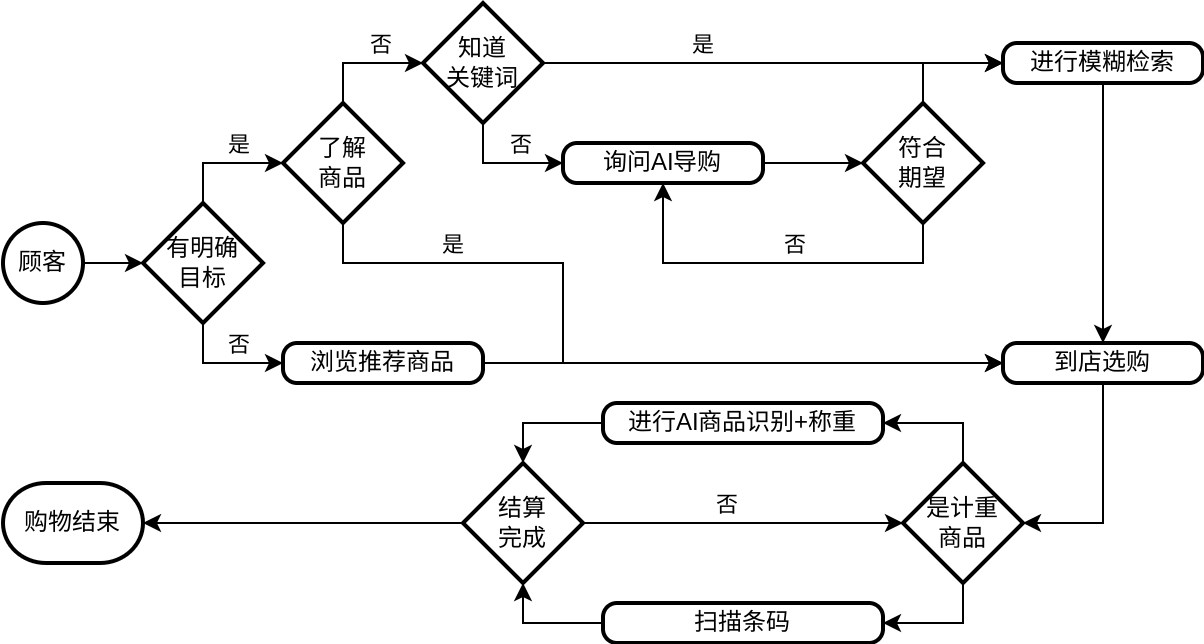
\includegraphics[width=0.8\textwidth]{./imgs/choose-n-buy.png}
	\caption{最终消费者商品选购流程}
	\label{fig:choose-n-buy}
\end{figure}

面向最终消费者的AI功能主要围绕着发现心仪商品和结算所购买商品的场景(如图 \ref{fig:choose-n-buy} 所示)展开。顾客发现商品的方式大致可以分为目的导向的和非目的导向的商品发现方式,其中非目的导向的商品发现方式与商户的宣传手段及其有效性关联较大,很大程度上取决于顾客是否浏览到该商铺对应宣传内容(实体、在线广告、客户群等)和对于宣传内容的实际吸引力。宣传内容的曝光可以由从业人员对社交媒体的参与来实现,而宣传内容可以借助上一部分提及的AI商品文案起草特性来辅助。目的导向的发现方式更为复杂。

目的导向的商品发现方式主要包括用户对商品进行搜索的过程。对于叫法比较单一、名称好记没有歧义的商品,简单分词---匹配的关键词搜索功能是可以满足需要的。然而,时间情况下商品名称匹配的问题可能远复杂于理想的情况。例如笼统和详细说法的区别:“可乐”和“苏打水”都可以叫作“汽水”,但这三个词语之间却无法直接相互匹配,并且若是为此将“汽水”拆为“汽”和“水”,不但仍然无法和“可乐”匹配,还可能会误匹配到与如“水”、“水汽”等词语相关的其他商品。

为了在一定程度上解决该问题,本设计包含模糊搜索引擎项目“探寻”及其对应词典处理脚本。该子项目采用“结巴”分词库\cite{sun_fxsjyjieba_2025,messense_messensejieba-rs_2025}进行分词,并且利用大语言模型对每个词语的近义词进行枚举,最后将各个来源的处理结果整理为高查询效率的格式在为中文优化的自定义搜索算法中进行部署,以此在消耗比较少的计算资源的情况下达到较高的搜索速度和(中文)搜索的准确率,有助于最终消费者更好地进行目的导向的商品发现活动,推动消费体验、营业质量提升。

然而性能更加强大的模糊搜索系统无法解决在许多情况下顾客不知悉需要搜索的关键词(及其近义词)的问题,这种情况下,顾客可能甚至并不清楚自己实际需要的商品。这个问题较为明显的解决思想是使得“商品发现”相关功能具有理解消费者对其需求的描述的语义并将需求内容对应于特定商品信息,或者为此生成对应的搜索语句提供给用户进行检索(或自动运行检索)。

为了解决这种情况带来的问题,该设计的顾客端移动应用程序包含AI导购助手模块。该模块利用经过特定提示词引导的多轮LLM对话及单次LLM调用,分别营造与顾客进行导购交流、导购向用户提出购买建议,如此往复的体验;从导购对用户的回复中提取出适用于检索的关键词语句,以此实现消费者只要合理形容需求,便可检索到对应商品的功能。

AI识别计重商品结算模块是该设计对一般传统实体零售流程的另一个改进。通过利用AI物体识别算法,在零售管理系统中整合物体识别AI模型的训练数据采集、标注等操作对应的用户界面,自动化模型训练和部署的过程;在结算终端中整合AI物体识别前端软件及摄像头、质量传感器等硬件来实现营业者轻松部署AI物体识别模型,最终用户轻松自助结算计重商品,去除计重商品结算过程对店员参与的要求。

\subsection{导购助手}

\begin{figure}[htbp]
	\centering
	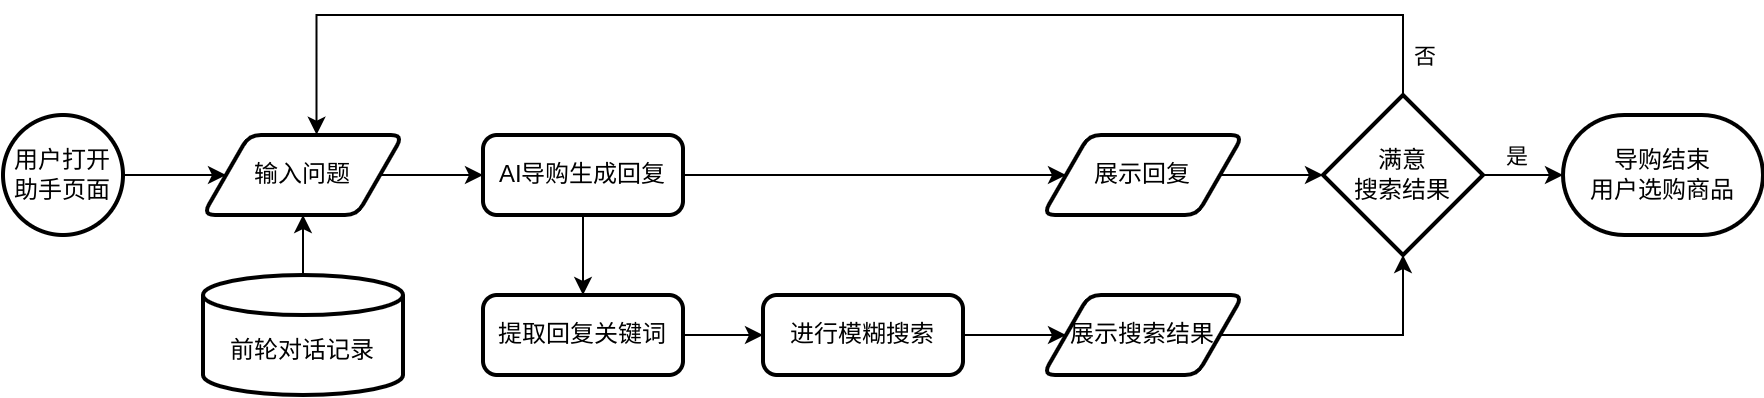
\includegraphics[width=0.8\textwidth]{./imgs/ask-n-choose.png}
	\caption{最终消费者导购操作流程}
	\label{fig:ask-n-choose}
\end{figure}

导购助手工作流程如图 \ref{fig:ask-n-choose} 所示,主要包括以下两个部分:

\begin{itemize}
    \item \textbf{对话式AI导购专家:} 通过与最终消费者的一轮或多轮对话确定消费者的具体需求,并给出相应的购买建议(商品类型、名称等)。
    \item \textbf{搜索关键词猜测算法:} 通过利用大语言模型强大的文字处理能力,使用AI导购的输出产生出对应的搜索关键词。
\end{itemize}

\subsubsection{对话型生成式AI}

AI导购专家实质上就是扮演导购身份,可以与用户进行多轮对话,解决用户困扰的人工智能聊天机器人(chatbot)。为了使得输出较为中性的无(行业相关)微调的一般大语言模型输出符合“导购身份”的回复,而不是一般的建议。该设计主要采用“百炼”的商业大模型 \verb|qwen-turbo| ,开发了以下的系统、对话提示模板:

\begin{itemize}
    \item[] \textbf{系统:}You are a helpful assistant of a retail shop that advise about buying stuffs.\footnote{此处为开发方便(并且遵照“百炼”官方文档中系统提示的风格)使用了英文系统提示,但实际测试中AI发挥了语言中性的能力,正确地使用中文响应了中文编写的输入。若需要中文提示,可以使用:你是零售商店的一个乐于助人的导购,你向客人提出购物建议。}
    \item[] (对每轮对话重复:)
    \begin{itemize}
        \item[] \textbf{用户:}\textit{(提出问题)}
        \item[] \textbf{模型:}\textit{(回复用户提问)}
    \end{itemize}
\end{itemize}

利用这样的对话模板,AI导购助手可以与用户进行(上下文长度范围内的)任意多轮对话,并且每轮对话之间可以产生关联(可以视为大模型聊天机器人的短时记忆特性),从而提高向用户提出正确推荐的概率。同时也因为对话记录参与下一轮对话的特性,应用程序带有由用户手动重置对话的功能,以此避免不同主题、结论的对话记录对新一轮对话大模型推理的干扰。

\subsubsection{搜索关键词提取}

在每一轮对话AI进行回复之后,相应的回复将会作为另一套提示词的一部分输入到模型中,以进行搜索使用的关键词的提取。在该设计对应实现中该特性使用的大模型为“百炼”的商业大模型 \verb|qwen-turbo| 。提示词对话如下:

\begin{itemize}
    \item[] \textbf{用户:}请根据这段话生成一些搜索商品的关键词,并且不要输出任何无关内容:\textit{(该轮对话中大模型的输出)}
\end{itemize}

理论上该过程可以和前文提及进行对话的过程进行合并,但该设计在此次选择将二者分开的设计方式,主要是有两个考量。首先是因为大模型输出难以控制格式的问题,此处避免需要大模型根据JSON等特定的格式输出结果(语义上就是输出两个不同的字符串),以此减轻对大模型推理、服从指引能力造成压力。其次是通过将大模型的输出输入到该任务的大模型(可以为同一个)之中,截断了单次全部输出的模式的标记(token)之间的线性关联,使得关键词的输出不直接受到用户原始输入(和前轮对话)的影响,从而一定程度上提高可预测性和防止模型受到用户特定语义不明确的输入而产生意外输出的问题。

\subsubsection{商品搜索}

\begin{figure}[htbp]
	\centering
	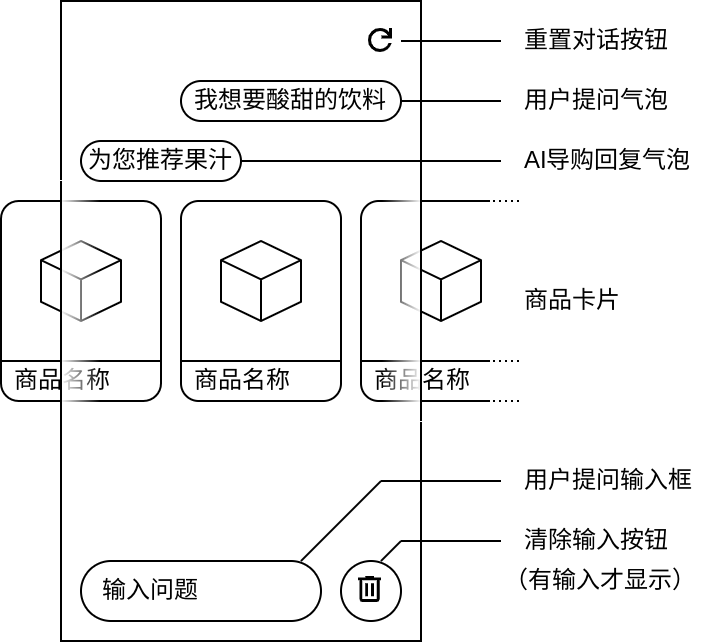
\includegraphics[width=0.8\textwidth, height=0.3\textheight, keepaspectratio]{./imgs/se-assist.png}
	\caption{AI导购用户界面}
	\label{fig:se-assist}
\end{figure}

大模型输出的关键词被用于模糊搜索,搜索结果连同用户的原始输入和AI导购的答复将经过如图 \ref{fig:se-assist} 所示的用户界面展示给用户。值得注意的是,前文提及的使得大模型提取AI导购回答中搜索关键词的输入之中并无对输出(搜索关键词)格式的规定。这是因为将在后文提及的模糊搜索算法是为词组而不是句子优化的,对实际上搜索语句的格式并无要求,仅仅只需要语句中包含期望的关键词。即便大模型忽视了引导(“关键词”)而输出了相关的连贯句子,搜索步骤也可以正常进行。

\subsection{称重商品识别}

在许多类型的零售细分领域中,不可避免地将会遇到按重量计算,而本身并无包装(俗称“散装”)的产品,这些商品包括但不限于在生鲜蔬果、米面粮油和零食糖果等多种类别中的产品。实际上在社会上的许多商场和超市中,消费者在选购这些“散装”商品的时候,由自己完成的步骤只能持续至商品的挑拣和包装。最为重要的称重环节必须由店员帮助完成,并且因为明显地许多这些商品本身无法贴上条码或其他标签,店员需要在容器上粘贴同时记录了商品类型和质量的“静态标签”或与结算系统联网同步的“动态标签”。这种方式既有重复度较高、专业性较低的人工辅助参与,又需要非标准(EAN-13)的商品信息传递记录手段。

为了缓解这个问题,本设计的结算系统包含利用摄像头和AI图像识别技术的智能计重商品结算功能,还配套用于收集、标记训练用数据的应用程序以简化识别模型的创建过程。借此称重设备的功能可以被整合到结算设备之中,使得用户可以轻松自主结算按质量计算价格的商品。

\subsubsection{数据准备}

\begin{figure}[htbp]
	\centering
	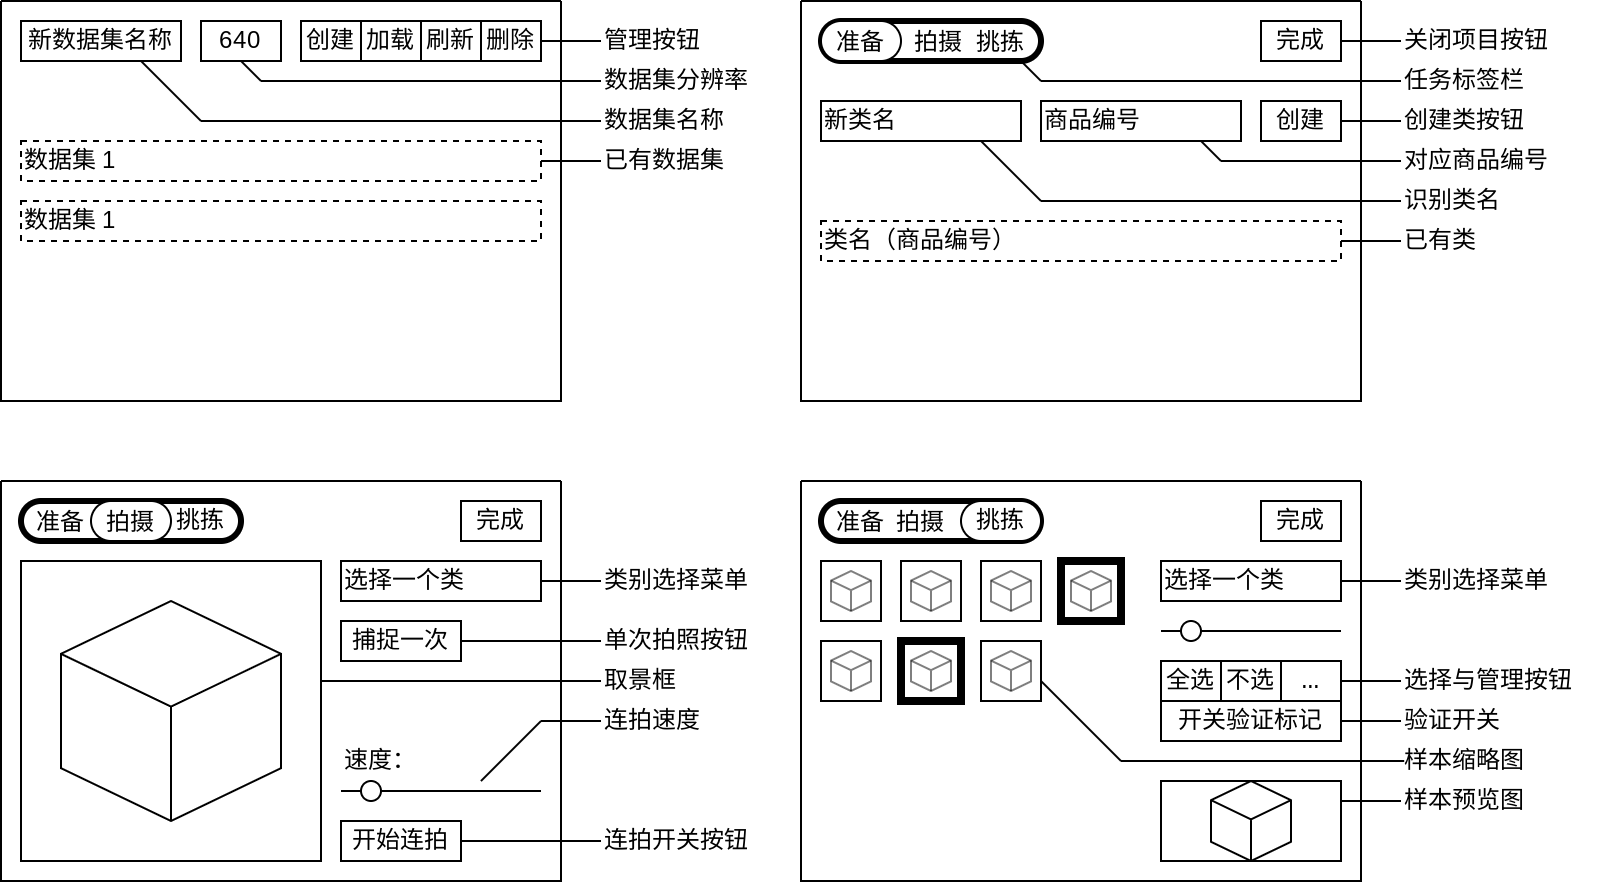
\includegraphics[width=0.8\textwidth]{./imgs/easydataset.png}
	\caption{“EasyDataset”数据集管理应用程序用户界面}
	\label{fig:easydataset}
\end{figure}

如图 \ref{fig:easydataset} 所示,从业者可以在“EasyDataset”应用程序内管理多个不同数据集。在应用程序内打开数据集之后,用户分别可以在“预备”、“拍摄”和“挑拣”三个标签页之间选择需要执行的操作。这三个操作一般情况下为递进顺序。

通过“预备”功能从业者可以准备需要AI识别模型检测到的商品类别列表,其中每个类别具有(隐藏的)类别编号、自身的名称和对应的商品编号。名称将被用于其余两个步骤中选择类别的参考,而商品编号将被用于模型实际部署的场景下结算系统将识别到的类别与具体商品联系起来的过程。此外,点击已经创建完毕的类别可以对其名称或者对应的商品编号进行修改。

使用“拍摄”功能可以为选定的类别拍摄图片。用户首先需要选择对应照片将保存到的类别,然后可以通过点击按钮来完成单张照片的拍摄。为了便于从业者在短时间之内拍摄大量不同角度的照片以提高识别模型的判别性能,该应用程序具有连拍功能。用户可以通过可拖动的调节组件调整连拍速度,其后通过点击按钮可以开始连拍。连拍的过程中用户可以不断调整商品的展示角度、摆放方式,而不需要关注用户界面方面的操作,再次点击按钮可以停止连拍。

针对选中类别,“挑拣”页面将展示已经拍摄的照片。在这个页面,从业者可以批量审阅拍摄完成的样本并从中去除图像素质不符合期望者,点击多个图片可以进行多选批量操作。此外,用户可以通过选中图片之后点击验证开关选择将一部分图片标记为模型效果验证(validation)用的图片,有助于在训练之后检测模型的泛化能力和预计效果。

\subsubsection{图像处理}

该应用程序并不直接保存拍摄的照片。为了考虑到训练和部署环境中可能的区别及数据集在不同版本的商品识别后端(或未来的新版本AI商品识别服务)之间的互换性(interoperability)和兼容性,数据集其中的商品图片统一裁切为以数据集定义时指定的边长的正方形。图片先被以二次线性(或其他更好的)插值算法重采样到短边与指定边长一致的相同长宽比新分辨率,再裁切其中央位置的最大正方形作为最终结果。这样,画面的内容被最大程度保留的同时对模型输入格式的要求较为宽松,并且通过(可选地)重采样到较低分辨率,训练的时间成本可以得到有效的控制,进一步降低使用门槛和维护成本。

\subsubsection{AI图像分类}

\begin{figure}[htbp]
	\centering
	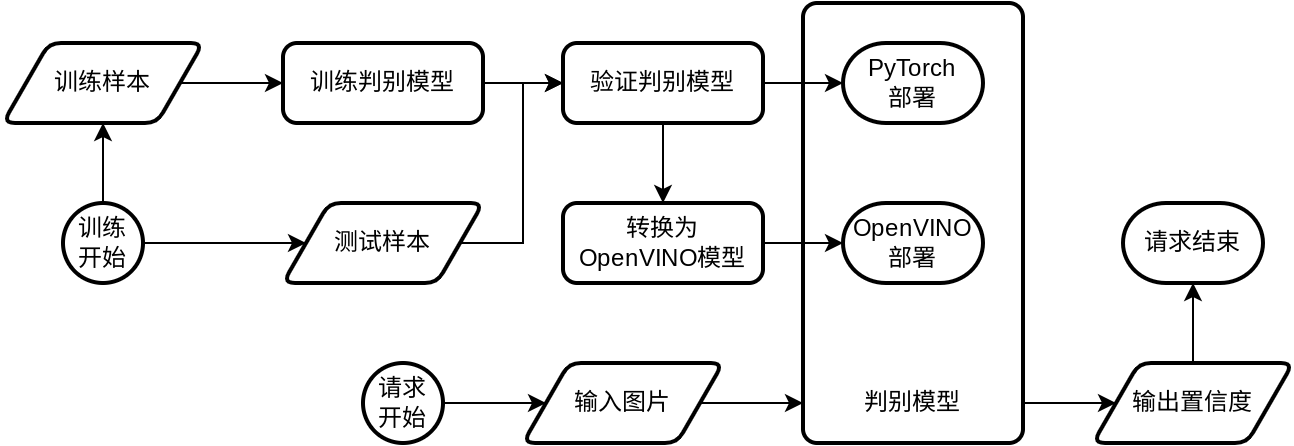
\includegraphics[width=0.8\textwidth]{./imgs/yolod.png}
	\caption{“yolod”图像分类训练-推理服务}
	\label{fig:yolod}
\end{figure}

该设计中提供AI图像分类、分类模型训练的服务“yolod”采用由ultralytics开发的YOLO11(版本 \verb|yolo11n-cls| )图像分类模型\cite{yolo11_ultralytics}作为模型架构,利用在CPU或(可选地)多种不同类型GPU上均可加速运行的PyTorch深度学习框架(版本2.6)和 \verb|ultralytics| 一体式YOLO开发辅助库进行训练和推理任务,利用FastAPI封装推理过程为HTTP API,结算终端应用程序只需要将编码过后的图片发送到yolod,服务器便会自动完成后续处理、推理工作并发回判别结果。

然而,直接使用主要为研究、开发场景优化的原生PyTorch模型进行推理任务效率是不够理想的,常常无法达到商品识别实时性的需要。为了解决这个问题,yolod包含透过\verb|ultralytics|展开的利用英特尔OpenVINO模型优化部署技术执行的推理后端,可以极大地提升推理的效率\footnote{前期实验中OpenVINO上部署的模型相比PyTorch在同样利用英特尔Arc A770 16GB加速硬件推理的情况下展现出了约11倍左右的性能提升。作者推测其中一部分提升幅度是PyTorch的SYCL(oneAPI Level Zero)后端在测试版本上缺乏优化引发的。},最大程度利用CPU或服务器所配置的兼容的加速硬件。值得一提的是,本设计鉴于特定的实验环境作出了使用OpenVINO的决定,但理论上任何有助于模型运行速度提升的部署方式(如ONNX、CoreML等)均可按情况进一步开发,投入使用。

\subsection{模糊搜索}

本设计所包含模糊搜索引擎“探寻”是一个以分词技术为基础,以大语言模型生成近义词作为词典拓展手段开发的、为中文优化的文本关键词模式匹配子系统。该子系统包括用于商品数据处理、AI近义词搜寻、词典构建的脚本和部署在第 \ref{sec:foundation} 部分的搜索算法四个部分。

\subsubsection{商品词典}

商品的搜索实质上是检测商品的标题或说明之中是否含有搜索语句相关模式(词语),同时匹配程度(模式命中次数)较高者更可能符合搜索语句对应语义。在这种情况下,任意一次命中于原文中的位置语义上并无作用,故输出匹配位置的字符串搜索算法并不适合该用途。同时,这也意味着可以快速检测模式是否存在而不包含模式位置相关信息的词典(dictionary)是最适合该用途的数据结构。为了更好传达算法的思想,现列出并解释下文将要直接使用的一些操作和类型:

\begin{itemize}
	\item $F_p$ \textbf{过滤(操作):}该操作接受一个字符串,并返回该字符串移除除了Unicode规范\cite{unicode16.0}所定义的拉丁文字(Latin)、汉字(Han)、假名(Hiragana、Katakana)和谚文(Hangul)以外的文字的版本。
	\item $F_e$ \textbf{扁平化(操作):}该操作接受一个由同元素类型可空集合组成的可空集合,并返回一个由所有原集合中子集合所包含的元素组成的新集合。
	\item $F_c$ \textbf{分词(操作):}该操作接受一个字符串,返回字符串的词语集合。
	\item \textbf{词典(类型):}以字符串(词语或标记)为键,以\textit{以编号数值为键,以频率数值为值的映射}为值的映射类型。
\end{itemize}

以下为根据标记(token)集合生成本模块对应词典数据的算法:

\vspace{1em}
\begin{algorithmic}
	\STATE \textbf{输入:}字符串的集合的序列 $x$
	\STATE \textbf{输出:}词典 $y$
	\STATE $y \gets \emptyset$
	\FOR {\textbf{each} $s$ \textbf{in} $x$ \textbf{of index} $i$}
		\FOR {\textbf{each} $c$ \textbf{in} $s$}
			\IF {$\nexists y(c)$}
				\STATE $y(c) \gets \emptyset$
			\ENDIF
			\IF {$\nexists y(c)(i)$}
				\STATE $y(c)(i) \gets 0$
			\ENDIF
			\STATE $y(c)(i) = y(c)(i) + 1$
		\ENDFOR
	\ENDFOR
\end{algorithmic}
\vspace{1em}

可见该算法遍历了每个条目(商品)对应的字符串(关键词),并对每个关键词在不同商品中的出现进行计数,以此来统计每个关键词与不同商品的关联程度。值得注意的是,该算法对每个商品的输入要求是关键词的集合,根据每个商品的名称和说明生成词语序列的算法如下:

\vspace{1em}
\begin{algorithmic}
	\STATE \textbf{输入:}商品名称和说明的二元组的序列 $x$
	\STATE \textbf{输出:}字符串的集合的序列 $y$
	\STATE $y \gets \emptyset$
	\FOR {\textbf{each} $(a, b)$ \textbf{in} $x$ \textbf{of index} $i$}
		\STATE $s \gets F_e(F_c(a) \cup F_c(b))$
		\STATE $s \gets \{F_p(x) \mid x \in s\}$
		\STATE $s \gets \{x \in s \mid x \neq \emptyset\}$
		\STATE $y \gets y \cup \{s\}$
	\ENDFOR
\end{algorithmic}
\vspace{1em}

由此可知该算法对商品的名称和说明都进行了分词操作,并将分词结果整合为一个序列,按输入的(商品)顺序进行分类,便于后续处理。

\subsubsection{AI近义词搜寻}

为了缓解上文提及的搜索算法无法理解搜索语句(及其单独词语)的语义从而无法搜索到意思相关的词语的问题,此处设计利用大语言模型优秀的自然语言处理能力进行前文提及的词典的拓展。考虑到词语数量可能较为庞大,云端处理的成本是较大的,此处使用本地部署的 \verb|qwen2.5-3b| 模型,提示词对话如下:

\begin{itemize}
	\item[] \textbf{用户:}输出这个词语的所有近义词为JSON字符串集合,不要输出无关内容:
	\item[](原词语)
\end{itemize}

通过在所有词语上重复该操作,并指定模型输出格式(schema)为JSON字符串数组,可以获得每个词语对应的近义词集合。此外,通过多次执行在所有词语上的遍历可以增加获得到的近义词集合的大小。值得注意的是,这种方法一定程度上依赖于模型对指令的遵从能力,并且生成的词语可能需要进一步分词、过滤操作才能用于后续处理。

\subsubsection{近义词词典}

现定义类型“近义词词典”为从词汇到其近义词集合的映射。为了便于实现搜索算法,现定义任何一个词语都是其本身的近义词,因此近义词词典的初始化方法是获取词典中的全部词语,并构建一个对全部词语,以该词语作为输入得到只有这个词语一个元素的集合的映射。生成近义词词典算法如下:

\vspace{1em}
\begin{algorithmic}
	\STATE \textbf{输入:}AI模型生成的近义词词典 $x_1$ ;词典 $x_2$
	\STATE \textbf{输出:}近义词词典 $y$
	\STATE $y \gets \emptyset$
	\FOR {\textbf{each key} $k$ \textbf{in} $x_2$}
		\STATE $y(k) \gets \{k\}$
	\ENDFOR
	\STATE $\hat{y} \gets \{x \mid \exists y(x), \lvert x \rvert \geq 4 \}$
	\FOR {\textbf{each key} $k$ \textbf{in} $y$}
		\STATE $\hat{y}_k \gets \{x \in \hat{y} \mid k \supset x \}$
		\STATE $y(k) \gets y(k) \cup F_e(\{y(x) \mid x \in \hat{y}_k\})$
	\ENDFOR
	\FOR {\textbf{each key} $k$ \textbf{in} $y$ \textbf{if} $\lvert k \rvert \geq 4$ \textbf{and} $x_1$}
		\FOR {\textbf{each} $v$ \textbf{in} $y(k)$}
			\IF {$\nexists y(v)$}
				\STATE $y(v) \gets \emptyset$
			\ENDIF
			\STATE $y(v) \gets y(v) \cup \{k\}$
		\ENDFOR
	\ENDFOR
\end{algorithmic}
\vspace{1em}

从算法上可以看到,首先 $y$ 被初始化为词语到其本身的映射,而后对任何字节长度大于4(一般可视为大于两个中文字符)的字符串,任何被其包含的其他词语对应的近义词都会被添加到该词语对应的近义词集合中(以弥补潜在分词不够细致的问题)。而后同样对任何字节长度大于4的词语其本身都将被添加到其每个近义词对应的近义词集合中,同时将会将这些词语添加为AI生成的近义词词典中对应近义词的近义词集合中。

\subsubsection{搜索算法}

在部署到服务器的搜索算法中,顾客发出的搜索语句首先会被分词和过滤,经过这些操作之后剩余的词语将会被用于实际匹配,搜索算法如下:

\vspace{1em}
\begin{algorithmic}
	\STATE \textbf{输入:}近义词词典 $s$ ;词典 $d$ ;搜索词集合 $x$
	\STATE \textbf{输出:}按匹配程度排序的商品编号序列 $y$
	\STATE $f \gets \emptyset$
	\FOR {\textbf{each} $w$ \textbf{in} $x$}
		\IF {$\exists s(w)$}
			\STATE \textbf{continue}
		\ENDIF
		\STATE $a \gets s(w)$
		\FOR {\textbf{each} $\hat{w}$ \textbf{in} $a$}
			\IF {$\exists d(\hat{w})$}
				\STATE \textbf{continue}
			\ENDIF
			\STATE $m \gets d(\hat{w})$
			\FOR {\textbf{each key} $k$ \textbf{in} $m$}
				\IF {$\exists f(k)$}
					\STATE $f(k) \gets 0$
				\ENDIF
				\STATE $f(k) \gets f(k) + m(k)$
			\ENDFOR
		\ENDFOR
	\ENDFOR
	\STATE \textbf{sort} $f$ \textbf{by value} 
	\STATE $y \gets \{x \mid \exists f(x)\}$
\end{algorithmic}
\vspace{1em}

对每个词语,首先从近义词词典查询其对应的近义词列表(由前文可知该列表可能包含该词语本身),若无结果,则说明该词语在所有商品文字的词语(及其近义词)中尚未出现,可以被安全忽略。否则,针对每一个近义词若词典之中有相应的项目其中所有商品编号对应的词频将会被累加到一个映射中,最后根据总词频对其进行排序,输出排序后的商品编号序列。